\documentclass[UTF-8,twoside,c5size]{ctexart}
\usepackage[dvipsnames]{xcolor}
\usepackage{amsmath}
\usepackage{amssymb}
\usepackage{geometry}
\usepackage{listings}
\usepackage{setspace}
\usepackage{xeCJK}
\usepackage{ulem}
\usepackage{pstricks}
\usepackage{pstricks-add}
\usepackage{bm}
\usepackage{mathtools}
\usepackage{breqn}
\usepackage{mathrsfs}
\usepackage{esint}
\usepackage{textcomp}
\usepackage{upgreek}
\usepackage{pifont}
\usepackage{tikz}
\usepackage{circuitikz}
\usepackage{caption}
\usepackage{tabularx}
\usepackage{array}
\usepackage{pgfplots}
\usepackage{multirow}
\usepackage{pgfplotstable}
\usepackage{mhchem}
\usepackage{graphicx}

\newcolumntype{Y}{>{\centering\arraybackslash}X}
\geometry{a4paper,centering,top=1.27cm,bottom=2.54cm,left=2cm,right=2cm}
\graphicspath{{figures/}}
\pagestyle{plain}
\captionsetup{font=small}

%\CTEXsetup[name={,.}]{section}
\CTEXsetup[format={\raggedright\heiti\noindent\zihao{-3}},numberformat={\bfseries}]{section}
\CTEXsetup[format={\raggedright\heiti\zihao{4}},numberformat={\bfseries}]{subsection}
\CTEXsetup[format={\raggedright\heiti\quad\zihao{-4}},numberformat={\bfseries}]{subsubsection}
\CTEXsetup[format={\raggedright\heiti\qquad},numberformat={\bfseries}]{paragraph}
\CTEXsetup[beforeskip=1.0ex plus 0.2ex minus .2ex, afterskip=1.0ex plus 0.2ex minus .2ex]{paragraph}
\renewcommand\thefootnote{\ding{\numexpr171+\value{footnote}}}

\setstretch{1.5}

\setCJKfamilyfont{boldsong}[AutoFakeBold = {2.17}]{SimSun}
\newcommand*{\boldsong}{\CJKfamily{boldsong}}
%\DeclareMathOperator\dif{d\!}
\newcommand*{\me}{\mathop{}\!\mathrm{e}}
\newcommand*{\mpar}{\mathop{}\!\partial}
\newcommand*{\dif}{\mathop{}\!\mathrm{d}}
\newcommand*{\tab}{\indent}
\newcommand*{\mcelsius}{\mathop{}\!{^\circ}\mathrm{C}}
\renewcommand*{\Im}{\mathrm{Im}\,}

\setcounter{secnumdepth}{4}

\renewcommand\arraystretch{1.5}

\lstset{
	backgroundcolor=\color[RGB]{245,245,245},
	keywordstyle=\color{blue}\bfseries,
	basicstyle=\small\ttfamily,
	commentstyle=\itshape\color{olive},
	numberstyle=\ttfamily,
	tabsize=4,
	breaklines=true
}

\begin{document}
	\begin{center}
		\heiti\zihao{-2}
		实验\textbf{6 $ \bm\sim $ 7}报告
	\end{center}

	\begin{table*}[!h]
		\raggedleft
		\zihao{-4}
		\begin{tabular}{ccc}
			{\heiti 学号} & {2019K8009929019} & {2019K8009929026} \\
			{\heiti 姓名} & 桂庭辉 & 高梓源 \\
			{\heiti 箱子号} & \multicolumn{2}{c}{44}
		\end{tabular}
	\end{table*}
	
	\section{实验任务}
	
	本次实验在流水线中添加部分普通用户态指令,主要包括9条算术逻辑运算类指令、7条乘除运算类指令、4条条件跳转指令、6条访存指令。这些指令中除乘除法外均可利用现有的数据通路,适当添加少量运算器件生成所需信号即可,主要的设计在于乘除法功能的自行实现
	
	\section{实验设计}	
	
	\subsection{总体设计思路}
	
	9条算术逻辑运算类指令的实现主要复用此前流水线中已实现的部分指令功能。\texttt{slti, sltui, andi, ori, xori}指令分别复用\texttt{slt, sltu, and, or, xor}指令数据通路,处理立即数内容与相关控制信号即可。\texttt{sll, srl, sra}指令分别复用\texttt{slli, srli, srai}指令数据通路,调整操作数来源与相关控制信号即可。\texttt{pcaddu12i}指令主要通路复用\texttt{add}指令,操作数处理上来自PC寄存器与\texttt{lu12i}指令结果。由于此部分几乎全部为对已有数据通路的复用,仅添加了部分控制信号,故而本篇报告中不再详述该部分的实现细节。
	
	% TODO:修改除法器实现
	% DONE::完成修改
	7条乘除法运算类指令中,乘法的处理我们使用自己编写的流水化乘法器,在两拍内计算出乘法结果;除法与取模的处理我们经历了三个设计阶段:(1)选择调用Xilinx IP定制除法器运算部件进行实现;(2)使用笔者自己完成的基于恢复余数法的迭代除法器;(3)使用经过加速迭代优化的除法器。除法运算的进行在ALU部件中完成,由于引入了新的运算与相关控制信号,需要维护流水级间的寄存器宽度、\texttt{alu\_op}宽度以及流水线控制的部分信号。
	
	4条条件转移指令的功能类比已实现的\texttt{beq、bne}指令,在译码级引入对大小的判断,具体大小判断的实现参考ALU中\texttt{slt}与\texttt{sltu}操作的实现。对转移信号的逻辑修改同样参考\texttt{beq、bne}指令即可。
	
	6条访存指令引入了单字节与半字长读写,已有框架中对\texttt{ld.w}与\texttt{st.w}实现的数据通路中的控制信号不足以应对新的情景,故而需要在流水槽中添加新的控制信号,包括访存地址低两位、访存宽度等信息,相应地在执行级修改数据RAM使能生成逻辑与访存级\texttt{load}结果生成逻辑。
	
	\subsection{重要模块设计:mul\_top与流水化后乘法实现}
	本小节所有模块设计均在tools.v文件中。
	\subsubsection{功能描述}
	
	乘法器顶层模块,例化17个数相加华莱士树模块\texttt{wallace}与33位Booth两位乘部分积生成器\texttt{boothgen}完成乘法器整体搭建与流水化。
	
	\subsubsection{工作原理}
	
	考虑硬件资源的节省,本次设计一个乘法器以完成有符号与无符号32位补码乘法。实现上如实验讲义所说将输入扩展成33位,通过33位补码乘法器实现对有无符号运算的同时支持。整体结构同样来自实验讲义。
	
	Booth两位乘部分积生成器的设计来自理论课教材,17个数相加的华莱士树设计来自实验课讲义。此处均不再赘述。在流水级划分上,考虑Booth部分积生成逻辑与华莱士树中6层1位全加器的总延迟约为20余级门(具体延迟大小取决于Vivado对1位加法器的实现),最终合并华莱士树结果的66位加法器将产生相当级别的延迟,故而选择将流水级切分在66位加法器入口处实现。采用一个133位寄存器将加法器的两个66位输入与1位进位输入锁一拍以实现流水化,在两拍内计算得到乘法结果。
	
	流水化的主要实现如下:
	\begin{lstlisting}[language=verilog]
	reg [132:0] bus;
	
	always @ (posedge clk) begin
		if (rst) begin
			bus <= 133'b0;
		end else begin
			bus <= {add_src1, add_src2, c[15]};
		end
	end
	
	assign res = bus[132:67] + bus[66:1] + {65'b0, bus[0]};\end{lstlisting}
	
	\subsubsection{接口定义}
	
	接口定义见下页。
	
	\begin{table}[!h]
		\centering
		\caption{乘法器顶层模块接口}
		\begin{tabularx}{\textwidth}{|c|c|c|Y|}
			\hline
			\textbf{名称} & \textbf{方向} & \textbf{位宽} & \textbf{描述} \\
			\hline
			\texttt{clk} & \textsc{In} & 1 & 时钟信号 \\
			\hline
			\texttt{rst} & \textsc{In} & 1 & 复位信号,高电平有效 \\
			\hline
			\texttt{mul\_signed} & \textsc{In} & 1 & 是否做有符号乘法 \\
			\hline
			\texttt{src1} & \textsc{In} & 32 & 源操作数1 \\
			\hline
			\texttt{src2} & \textsc{In} & 32 & 源操作数2 \\
			\hline
			\texttt{res} & \textsc{Out} & 64 & 乘法运算结果 \\
			\hline
		\end{tabularx}
	
		\caption{华莱士树模块接口}
		\begin{tabularx}{\textwidth}{|c|c|c|Y|}
			\hline
			\textbf{名称} & \textbf{方向} & \textbf{位宽} & \textbf{描述} \\
			\hline
			\texttt{in} & \textsc{In} & 17 & 待相加的17个1位数 \\
			\hline
			\texttt{cin} & \texttt{In} & 14 & 来自先前华莱士树或转置部件的进位输入 \\
			\hline
			\texttt{cout} & \textsc{Out} & 14 & 传递给后续华莱士树的进位输入 \\
			\hline
			\texttt{carry} & \textsc{Out} & 1 & 压缩结果:进位输出 \\
			\hline
			\texttt{sum} & \textsc{Out} & 1 & 压缩结果:和 \\
			\hline
		\end{tabularx}
	
		\caption{部分积生成模块接口}
		\begin{tabularx}{\textwidth}{|c|c|c|Y|}
			\hline
			\textbf{名称} & \textbf{方向} & \textbf{位宽} & \textbf{描述} \\
			\hline
			\texttt{y} & \textsc{In} & 3 & 来自乘数的部分积生成标志信号 \\
			\hline
			\texttt{x} & \textsc{In} & 66 & 移位处理后的被乘数 \\
			\hline
			\texttt{c} & \textsc{Out} & 1 & 部分积的末位进位输入(取反“加一”) \\
			\hline
			\texttt{p} & \textsc{Out} & 66 & 部分积 \\
			\hline
		\end{tabularx}
	\end{table}

	\subsubsection{乘法实现的其他逻辑}
	
	由于乘法器与其他运算逻辑一样集成到ALU部件中,而流水化后的乘法指令为了避免影响流水线性能,应如访存指令一样在指令进入流水级时取得乘法结果,为了实现该功能,需要将乘法运算结果导出至执行级外传递给访存级。乘法实现里引入的时序逻辑除此前介绍的乘法计算中的流水级切分外,乘法所需结果是高32位还是低32位所需的控制信号也需要时序逻辑保存到下一拍,即乘法指令位于访存级时。该信号的传递可以通过执行级与访存级间的流水槽实现,也可以单独缓存该信号利用传递乘法结果的通路进入访存级参与结果选择。
	
	此外,由于乘法指令与访存指令一样,在访存级才能得到写回结果,故而如访存指令一样,也需在前递机制中引入乘法指令于执行级与译码级指令冲突时的阻塞信号。
	
	% TODO:除法器设计修改
	\subsection{除法器IP调用与时序处理}
	
	笔者将乘除法所有实现放在alu.v中,这就意味着alu\_op需要拓宽至19位,囊括所有乘除法指令信息,对于除法需要有无符号的信息、取商或余数的信息,并且这些信息彼此互斥,很难提取共同特征而缩减,因此可直接对乘除法每类指令设置一位alu\_op,求得的结果也可以根据alu\_op直接选取。
	
	\subsubsection{接口定义}
	
	根据讲义描述,调用并设置好Vivado提供的有无符号除法IP核,注意IP核暴露的所有接口都有作用,需要全部连接,接口如下页。
	
	\begin{table}[!h]
	\begin{center}
		\caption{除法器IP核接口定义}
		\begin{tabularx}{\textwidth}{|c|c|c|Y|}
			\hline
			\textbf{接口} & \textbf{I/O} & \textbf{位宽} & \textbf{说明} \\
			\hline
			\texttt{aclk} & \textsc{In} & 1 & 时钟驱动,迭代除法 \\
			\hline
			\texttt{s\_axis\_divisor\_tdata} & \textsc{In} & 32 & 除数输入 \\
			\hline
			\texttt{s\_axis\_dividend\_tdata} & \textsc{In} & 32 & 被除数输入 \\
			\hline
			\texttt{s\_axis\_divisor\_tready} & \textsc{Out} & 1 & 是否准备好读取除数 \\
			\hline
			\texttt{s\_axis\_dividend\_tready} & \textsc{Out} & 1 & 是否准备好读取被除数 \\
			\hline
			\texttt{s\_axis\_divisor\_tvalid} & \textsc{In} & 1 & 除数输入是否有效,开始运算 \\
			\hline
			\texttt{s\_axis\_dividend\_tvalid} & \textsc{In} & 1 & 被除数输入是否有效,开始运算 \\
			\hline
			\texttt{m\_axis\_dout\_tdata} & \textsc{Out} & 64 & 商和余数结果输出 \\
			\hline
			\texttt{m\_axis\_dout\_tvalid} & \textsc{Out} & 1 & 输出是否有效,当前除法是否算完 \\
			\hline
		\end{tabularx}
	\end{center}
	\end{table}

	\subsubsection{使用说明}
	\label{Valid_input}

	正如讲义强调的,除法IP核采用AXI总线接口,Ready和Valid信号同时有效时开始输入,经过观察,我们设置的clocks per Division选项是Ready信号每次拉高间隔的时钟周期数,我们需要保证Valid信号第一次和Ready信号同时拉高后必须在该除法计算整个完成后(m\_axis\_dout\_tvalid信号拉高)之后才能有条件再度拉高,进行下一次计算,在此过程中流水级也需要进行阻塞。
	
	笔者在实验中使用了另一个信号div\_valid,它为高电平当且仅当整个除法运算开始且未结束,于是一旦它为高电平,除法器输入的两个Valid信号就不能拉高。因为除数被除数的Ready和Vallid信号需要同时拉高,用同一个div\_data\_valid信号进行控制即可,于是下面是控制信号的时序赋值过程:
	
	\begin{lstlisting}[language=verilog]
	always @(posedge clk) begin
		if (div_valid) begin
			div_data_valid <= 1'b0;
		end else if (es_valid & use_div & (~divisor_data_ready | ~dividend_data_ready)) begin
			div_data_valid <= 1'b1;
		end else begin
			div_data_valid <= 1'b0;
		end
		
		if (div_valid) begin
			divu_data_valid <= 1'b0;
		end else if (es_valid & use_divu & (~u_divisor_data_ready | ~u_dividend_data_ready)) begin
			divu_data_valid <= 1'b1;
		end else begin
			divu_data_valid <= 1'b0;
		end
		
		if (rst) begin
			div_valid <= 1'b0;
		end else if (div_res_valid | divu_res_valid) begin
			div_valid <= 1'b0;
		end else if ((div_data_valid & divisor_data_ready) | (divu_data_valid & u_divisor_data_ready)) begin
			div_valid <= 1'b1;
		end
	end
	\end{lstlisting}

	除法器实例化连接后,对于结果直接取$[63:32]$位作为商,$[31:0]$作为余数。
	
	\subsection{自行设计实现除法器}
	
	\subsubsection{功能描述}
	
	根据讲义的方法,按照绝对值恢复余数除法,设计实现了固定34个时钟周期完成有无符号除法运算的除法器。
	
	\subsubsection{接口定义}
	
	因为首先单独设计除法器,使用给出的test\_bench.v进行正确性验证,因此接口定义按照test\_bench.v的调用方式,在alu中使用也按照相同的方式。接口如下:
	
	\begin{table}[!h]
		\begin{center}
			\caption{自行设计除法器接口定义}
			\begin{tabularx}{\textwidth}{|c|c|c|Y|}
				\hline
				\textbf{接口} & \textbf{I/O} & \textbf{位宽} & \textbf{说明} \\
				\hline
				\texttt{clk} & \textsc{In} & 1 & 时钟驱动,迭代除法 \\
				\hline
				\texttt{rst} & \textsc{In} & 1 & 复位信号,重新开始除法 \\
				\hline
				\texttt{div} & \textsc{In} & 1 & 是否开始进行除法 \\
				\hline
				\texttt{div\_signed} & \textsc{In} & 1 & 是否采用有符号除法 \\
				\hline
				\texttt{x} & \textsc{In} & 32 & 被除数输入 \\
				\hline
				\texttt{y} & \textsc{In} & 32 & 除数输入 \\
				\hline
				\texttt{s} & \textsc{Out} & 32 & 商结果输出 \\
				\hline
				\texttt{r} & \textsc{Out} & 32 & 余数结果输出 \\
				\hline
				\texttt{complete} & \textsc{Out} & 1 & 输出是否有效,当前除法是否算完 \\
				\hline
			\end{tabularx}
		\end{center}
	\end{table}

	\paragraph{使用实例}\hfill
	
	举出在alu中使用该除法器替代IP核除法器的示例,注意可以将AXI总线相关控制逻辑删除。
	
	\begin{lstlisting}[language=verilog]
		divider alu_div(
			.clk(clk),
			.rst(rst),
			.div(is_div),
			.div_signed(use_div),
			.x(alu_src1),
			.y(alu_src2),
			.s(div_result),
			.r(mod_result),
			.complete(div_finish)
		);
	\end{lstlisting}

	\subsubsection{工作原理}
	
	\paragraph{绝对值处理}\hfill
	
	首先对有符号除法运算中负数取绝对值后统一做无符号运算,记录这一信息,最后再由讲义提供的符号位规则表进行恢复:
	
	\begin{lstlisting}[language=verilog]
		// at beginning
		wire [31:0] X;
		wire [31:0] Y;
		
		wire dividend_sign  = div_signed & x[31];
		wire divisor_sign   = div_signed & y[31];
		wire s_sign         = dividend_sign ^ divisor_sign;
		wire r_sign         = dividend_sign;
		
		assign X[31:0]      = (dividend_sign ? ~x[31:0]+1 : x[31:0]);
		assign Y[31:0]      = (divisor_sign  ? ~y[31:0]+1 : y[31:0]);
		
		// in the end
		assign s[31:0] = s_sign ? ~S[31:0] + 32'b1 : S[31:0];
		assign r[31:0] = r_sign ? ~dividend_w[31][31:0] + 32'b1 : dividend_w[31][31:0];
	\end{lstlisting}

	\paragraph{准备时序迭代}\hfill
	
	思路很简单,因为核心模块为在滑动窗口内完成减法,每次的结果充当下一次输入,因为要符合时序,满足多周期完成除法,因此使用reg类型数组作为每次例化的输入,wire类型数组作为每次例化输出,每当时钟上升沿可以更新上层迭代时即可将wire结果赋值到下一层的reg输入。以变量\texttt{time\_i}作为开始和结束以及每一轮进行迭代层数的标志。
	
	\begin{lstlisting}[language=verilog]
		reg [5:0] time_i;
		always @(posedge clk) begin
			if(rst) begin
				time_i <= 0;
			end else if(time_i != 6'd33 && div) begin
				time_i <= time_i + 5'b1;
			end else begin
				time_i <= 0;
			end
			
			if(time_i == 0 || time_i == 1) begin
				dividend_r[0][63:0]    <= {32'b0, X[31:0]};
			end else begin
				dividend_r[time_i[5:0]-1][63:0] <= dividend_w[time_i[5:0]-2][63:0];
			end
		end
		
		genvar i;
		generate
			for(i = 0; i < 32; i = i + 1) begin
				minus div_minus(.A(dividend_r[i]), .B(divisor),.shift(i),.S(S[31-i]),.new_A(dividend_w[i]));
			end
		endgenerate
	\end{lstlisting}

	\paragraph{滑动窗口迭代逻辑}\hfill
	
	根据恢复余数法,每次扩展被除数的滑动窗口与扩展除数做减法,若结果为负数,则说明不够减,商对应位置为0,仍然用被除数进行下一次减法;若结果为正数,则说明够减,商对应位置为1,此时将余数更新到滑动窗口,提供给下一次减法。
	
	在笔者的设计中,为方便在模块例化时使用\texttt{generate},需要避免位拼接操作,使用\texttt{shift}替代。每次传入和输出都可以直接为64位,也方便了时序赋值,而在减法模块中,使用\texttt{src1}作为被除数33位的滑动窗口,更新结果时使用\texttt{clear, res\_assign},前者清除被除数对应位置,后者将减法的33位结果移到对应窗口位置,进行先与后或即可完成。
	
	\begin{lstlisting}[language=verilog]
		module minus (
		input   [63: 0]     A,
		input   [32: 0]     B,
		input   [ 6: 0]     shift,
		output              S,
		output  [63: 0]     new_A
		);
		
			wire [32: 0]    src1;
			wire [63: 0]    src1_mid;
			wire [32: 0]    res;
			wire [63: 0]    clear;
			wire [63: 0]    res_assign;
			
			assign src1_mid = A[63:0] << shift;
			assign src1 = src1_mid[63:31];
			assign res = src1[32: 0] - B[32: 0];
			
			assign S = ~res[32];
			
			assign clear[63:0] = (S ? ((shift == 7'b0) ? {33'b0,31'h7fffffff} : {1'b1,33'b0,30'h3fffffff} >>> (shift-1)) : 64'hffffffff);
			
			assign res_assign[63:0] = (S ? {31'b0, res[32:0]} << (31-shift) : 64'b0);
			
			assign new_A = (A & clear | res_assign);
		endmodule
	\end{lstlisting}

	\paragraph{除法完成判断}\hfill
	
	既然reg型变量\texttt{time\_i}代表当前迭代层数,因此当层数达到,数组填充、商最低位计算完成后即可拉高\texttt{complete}:
	
	\begin{lstlisting}[language=verilog]
		assign complete = (time_i == 6'd33);
	\end{lstlisting}

	\paragraph{仿真时序结果}\hfill
	
	\begin{figure}[!h]
		\centering
		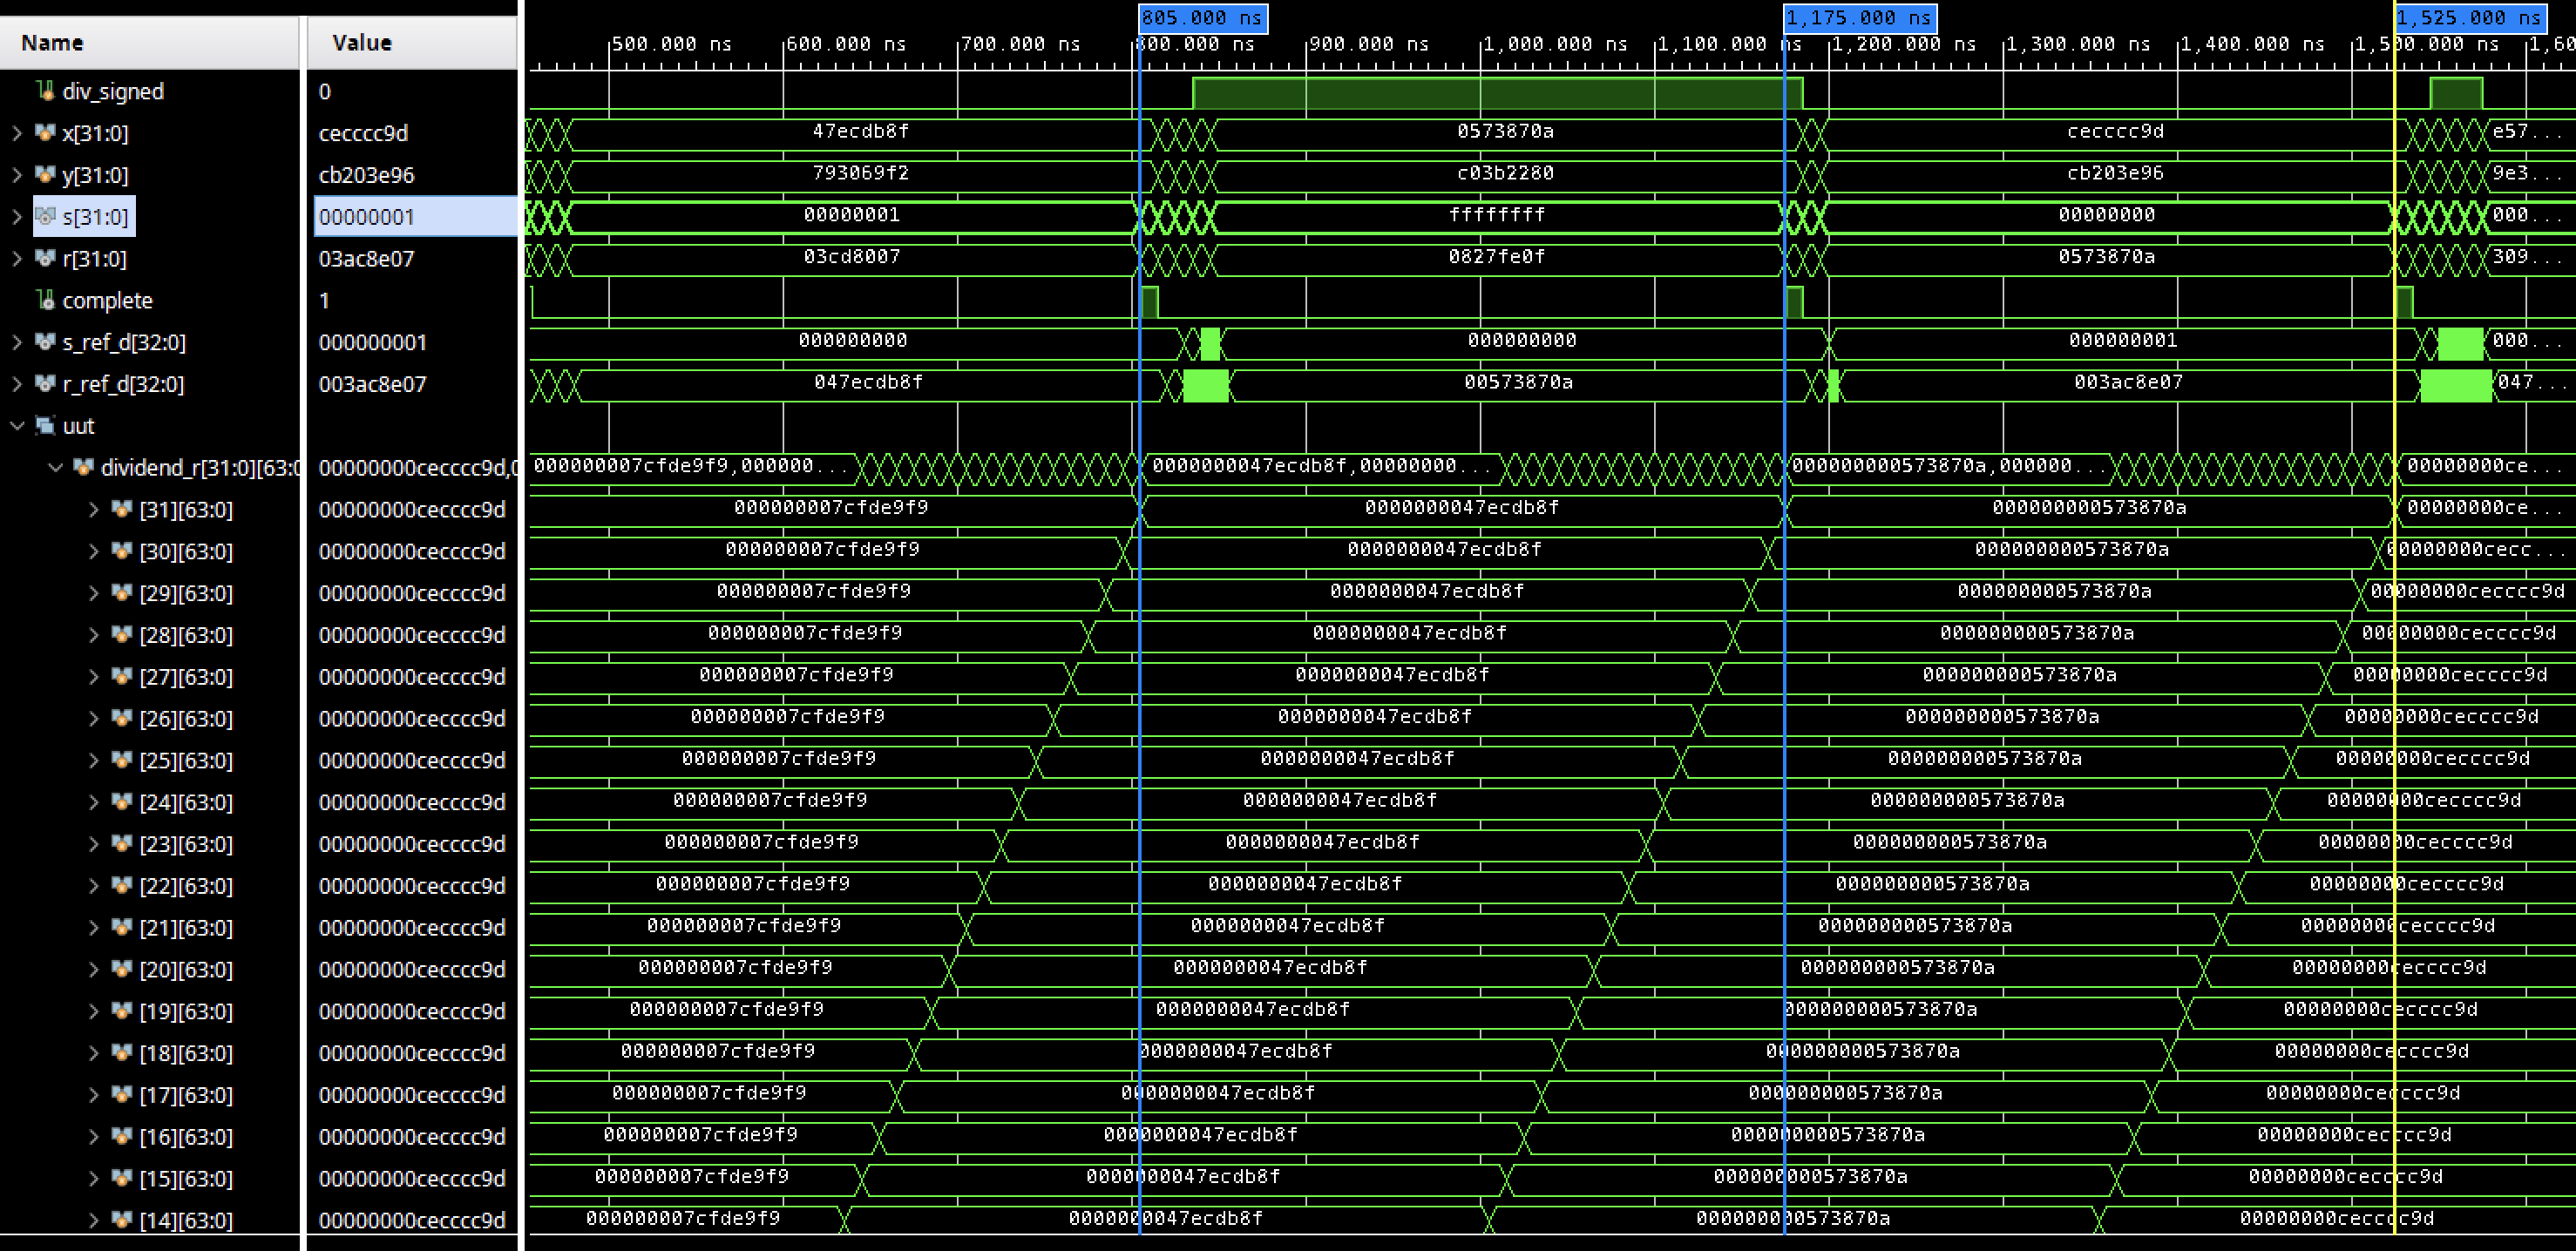
\includegraphics[width=1\linewidth]{figures/div_DIY.png}
		\caption{自行设计除法器仿真时序结果}
		\label{fig:divdiy}
	\end{figure}

	\subsection{除法器优化}
	
	\subsubsection{功能描述}
	
	由仿真时序图\ref{fig:divdiy}可以明显看到,按照讲义给出的算法,由于被除数前添加32个0,最初滑动窗口形成的被减数很小,在一般的概率条件下,直到很多轮迭代之后才可能和减数具有相同大小,出现1为结果、使用减法结果替换滑动窗口的情况,在此之前,扩展被除数并不会改变。因此,优化方向便是需要提前开始有意义(以1为结果)的减法,在得到正确结果后提前结束。
	
	由于只是在除法器顶层模块修改算法,并不需要改变接口,接口定义与使用方法与上相同。
	
	\subsubsection{工作原理}
	
	\paragraph{寻找最高有效位}\hfill
	
	所谓有效位即为1的位置。由以上对于优化方向的简述,我们需要定位何时被减数能够与减数“相抗衡”,即最高有效位在同一位置。笔者使用二分法进行迭代,十分巧妙找出最高有效位。
	
	\begin{lstlisting}[language=verilog]
		module find_64 (
			input   [63: 0]    x,
			output  [ 5: 0]    y
		);
		
			wire [31: 0]    data_32;
			wire [15: 0]    data_16;
			wire [ 7: 0]    data_8;
			wire [ 3: 0]    data_4;
			wire [ 1: 0]    data_2;
			
			assign y[5] = |x[63:32];
			assign data_32 = y[5] ? x[63:32] : x[31:0];
			assign y[4] = |data_32[31:16];
			assign data_16 = y[4] ? data_32[31:16] : data_32[15:0];
			assign y[3] = |data_16[15:8];
			assign data_8  = y[3] ? data_16[15:8] : data_16[7:0];
			assign y[2] = |data_8[7:4];
			assign data_4  = y[2] ? data_8[7:4] : data_8[3:0];
			assign y[1] = |data_4[3:2];
			assign data_2  = y[1] ? data_4[3:2] : data_4[1:0];
			assign y[0] = data_2[1];
		endmodule
	\end{lstlisting}

	这里以64位算法为例,因为需要频繁位操作以及需要使用对数函数展开,不方便使用\texttt{generate}或者利用\texttt{parameter}做出一个具有通用性的查找器。如上代码所示,每次进行左右二分,进行按位或,将结果对应位置位,而后取左半或者右半作为下一次迭代的输入即可。
	
	\paragraph{一次性初始化赋值加速迭代}\hfill
	
	得到被除数和除数最高有效位位置的差\texttt{skip\_pos}之后,可以一次性赋值迭代减法器输入数组的低\texttt{skip\_pos}位,这里放在时序逻辑中使用\texttt{for}循环完成赋值,需要注意某些边界问题,比如是否可以加速的位数超过了32,即数组的容量。但有些边界是模糊的,与优化的程度好坏有关。
	
	\begin{lstlisting}[language=verilog]
		reg  [ 5: 0]    time_i;
		reg  [ 5: 0]    time_j;
		reg  [ 1: 0]    time_i_added;
		reg             dividend_added;
		always @(posedge clk) begin
			if(rst || complete) begin
				time_i <= 0;
				time_i_added <= 0;
				dividend_added <= 0;
			end else if(time_i != 6'd33 && div && ~time_i_added[0] && ~time_i_added[1]) begin
				time_i_added <= time_i_added + 2'b1;
			end else if(time_i != 6'd33 && div && time_i_added[0]) begin
				time_i <= skip_pos;
				time_i_added <= time_i_added + 2'b1;
			end else if(time_i != 6'd33 && div && (time_i_added[1] & ~time_i_added[0])) begin
				time_i <= time_i + 1;
			end else begin
				time_i <= 0;
			end
			
			if(time_i == 0) begin
				dividend_r[0][63:0]    <= {32'b0, X[31:0]};
			end else if(!dividend_added) begin
				for(time_j = 1; time_j <= skip_pos && time_j < 6'd32 ; time_j = time_j + 1) begin
					dividend_r[time_j[4:0]][63:0] <= {32'b0, X[31:0]};
				end
				dividend_added <= 1'b1;
			end else if(time_i != 6'd32) begin
				dividend_r[time_i[4:0]][63:0] <= dividend_w[time_i[4:0]-1][63:0];
			end
		end
	\end{lstlisting}

	上述代码中所谓\texttt{time\_j}所在的循环语句即为加速赋值的核心语句,注意在加速赋值结束之后,仍然需要按照原先正常的除法器时序往下走,因此对\texttt{time\_i},增加了一个2位的变量来判断当前状态,若刚进行初始化,则增1开始除法,若未加速赋值,则跳转到赋值后的迭代层,若已加速赋值,则每拍增1,直到完成除法。
	
	\paragraph{仿真时序图}\hfill
	
	\begin{figure}[h]
		\centering
		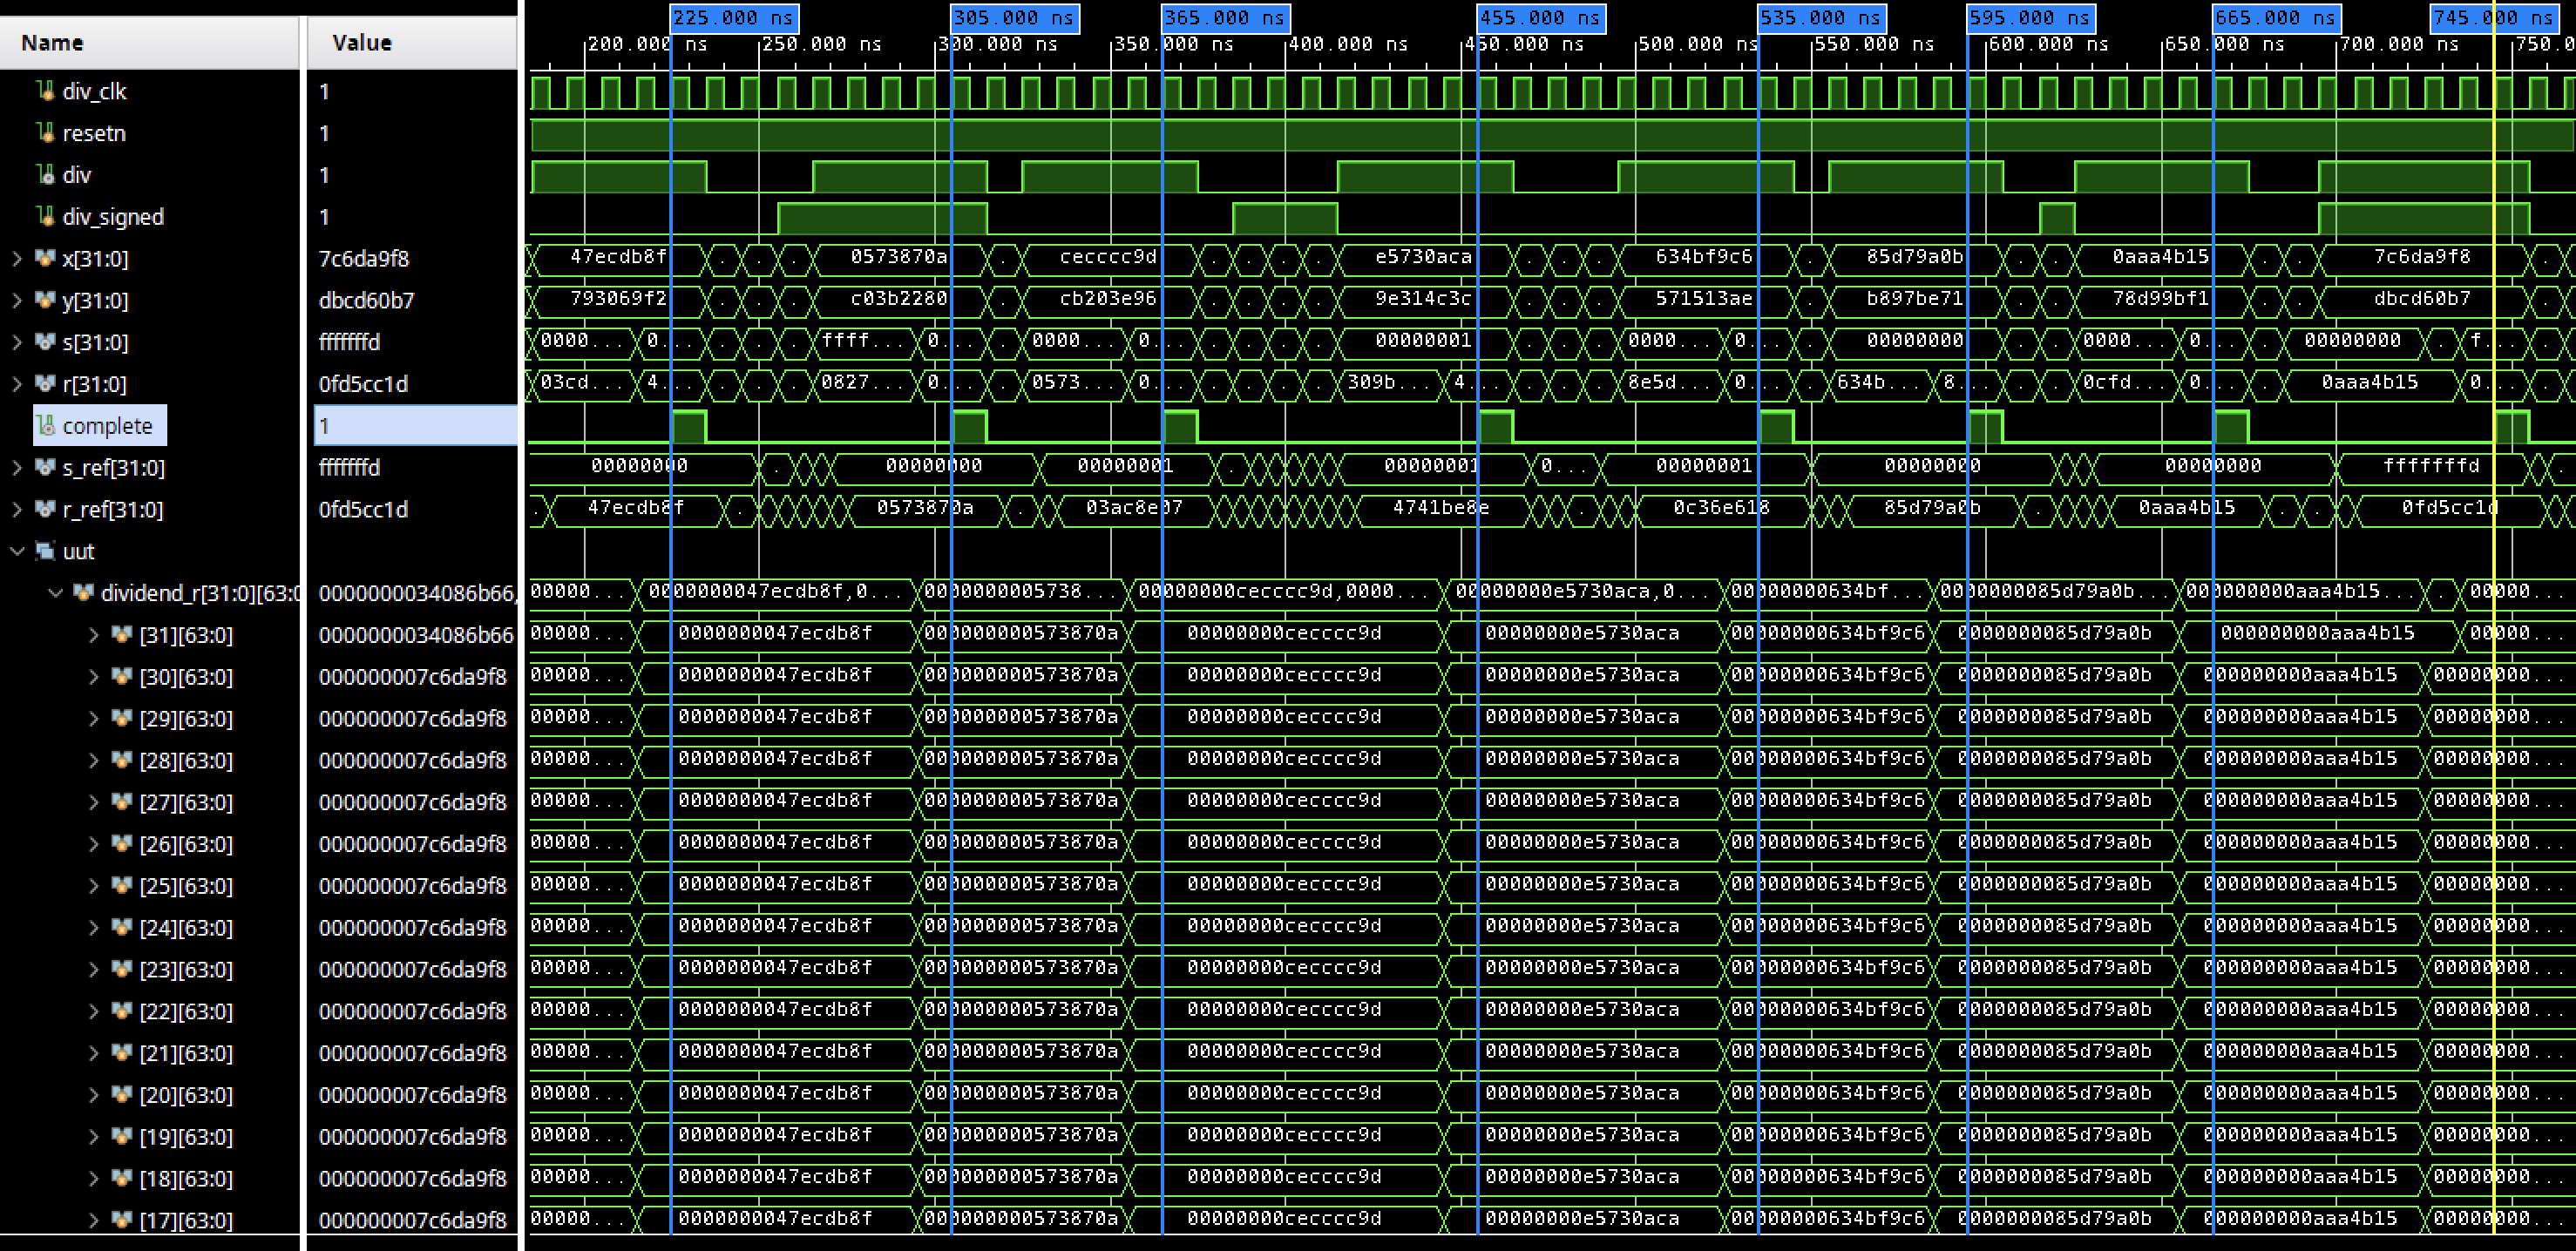
\includegraphics[width=1\linewidth]{figures/div_acc.png}
		\caption{加速后除法器仿真时序结果}
		\label{fig:divacc}
	\end{figure}

	通过仿真结果发现,优化后除法器平均8拍即可完成一次除法,性能提升3倍有余。
	
	
	\subsection{转移指令的添加}
	增添的四条转移指令为\texttt{blt, bge, bltu, bgeu},需添加有无符号下的$ < $判断,$ \geqslant $结果对$ < $结果取反即可。
	
	基于现有的流水线框架,上述判断的实现仍在译码级完成,显然ALU中已实现相同功能(\texttt{slt, sltu}),译码级完成会导致硬件资源的浪费。在不修改流水级控制与\texttt{alu\_op}生成逻辑的基础上,为减少这样的浪费,参考本课程ALU的实现与计算机组成原理实验课中ALU的设计,使用一个34位加法器计算两待比较数据的差,通过符号位得到有符号比较结果,通过借位信号得到无符号比较结果。
	
	\begin{lstlisting}[language=verilog]
	assign {regs_minus_carry, regs_minus_res, regs_minus_low}
		= {1'b1, rj_value, 1'b1} + {1'b0, ~rkd_value, 1'b1};
	assign rj_lt_rd = (rj_value[31] & ~rkd_value[31]) |
					 ((rj_value[31] ^~ rkd_value[31]) & regs_minus_res[31]);
	assign rju_lt_rdu = regs_minus_carry;
	\end{lstlisting}

	由此已获得了类似\texttt{beq, bne}中的\texttt{rj\_eq\_rd}判断结果,类比这两条指令在\texttt{br\_taken, br\_target}逻辑中进行修改即可。
	
	\subsection{访存指令的添加}
	
	如前文所述,需对新访存指令的支持需要让执行级与访存级获得更多的控制信息,故而我们扩展已有的\texttt{load\_op}信号,增添\texttt{store\_op}信号,将访存指令译码结果传递给后续流水级而非原先单比特的选择控制信号\texttt{mem\_from\_mem}。
	
	执行级的数据RAM输入信号中,数据RAM使能与访存地址的逻辑与此前基本一致,只是前者需要适应新的流水槽信息,后者注意对齐\footnote{实践表明,此处不做对齐处理也能正确执行,说明在数据RAM的实现中对输入的地址进行了对齐处理。}。字节写使能与写数据的逻辑需要进行修改。字节写使能对\texttt{st.w}而言是全1;对于\texttt{st.b}而言是根据访存地址低两位的数值在对应位上置1,该操作可通过移位器实现;对于\texttt{st.h}而言则类似\texttt{st.b},根据访存地址在高低两位中选择地置1。基于这样的字节写使能,对数据RAM而言字节写使能拉低处的字节数据是未定义的,所以简化写数据逻辑,对不同写宽度下直接按宽度扩展待存数据即可。
	
	访存级处理数据RAM读端口的读取结果,根据\texttt{load\_op}可获得读取宽度、有无符号扩展信息,基于这些可构建一个三路选择器:
	\begin{lstlisting}[language=verilog]
assign load_result = {32{load_byte}} & {{24{load_b_data[7] & load_signed}},load_b_data} |
		{32{load_half}} & {{16{load_h_data[15] & load_signed}},load_h_data} |
		{32{load_word}} & mem_result;
	\end{lstlisting}
	其中\texttt{load\_b\_data}与\texttt{load\_h\_data}为根据ALU计算出的访存地址从读端口给出的4字节数据中截取指定字节或半字的结果。
	
	\section{实验过程}
	
	\subsection{实验流水账}
	
	2021.09.30 08:00 $\sim$ 2021.09.30 09:00 :完成第一部分,对9条算术逻辑类指令的实现
	
	2021.10.01 14:00 $\sim$ 2021.10.01 16:00 :利用Xilinx IP完成乘除法指令实现
	
	2021.10.02 15:00 $\sim$ 2021.10.02 16:45 :完成流水化乘法器支持乘法指令
	
	2021.10.04 20:00 $\sim$ 2021.10.04 23:00 :完成自行设计的除法器支持除法与取模指令
	
	2021.10.05 13:00 $\sim$ 2021.10.05 15:00 :完成转移与访存指令添加
	
	% TODO:实验报告撰写时间
	2021.10.11 18:00 $\sim$ 2021.10.12 00:00 :撰写实验报告
	
	\subsection{错误记录}	
	\subsubsection{错误\textbf{1:}流水化后乘法结果获取出错}
	\paragraph{错误现象}\hfill
	
	%	四级节标题后面的\hfill与空行不可省略,不然节内容会跟着标题,目前我也只会这方法处理
	
	对于乘法指令,在访存级获取到的计算结果为0。
	
	\paragraph{分析定位过程}\hfill
	
	无论是访存级还是执行级,其中获取到的乘法结果均为0,但乘法器结果正确,说明问题来自ALU中对乘法结果的处理。
	
	\paragraph{错误原因}\hfill
	
	在最初的设计中,我们在ALU中根据\texttt{alu\_op}译码结果对乘法结果的高低位进行选择,然后传递32位数据给访存级,这一过程的“选择”使用与或逻辑实现,同时该选择过程为纯组合逻辑。那么在乘法指令进入访存级时,下一条指令进入执行级,\texttt{op\_mul}等乘法译码结果均被拉低,导致选择器结果为0无意义。
	
	\paragraph{修正效果}\hfill
	
	注意到选择信号的时序问题,我们选择引入寄存器保存高低选择信号至下一拍,同时传递的乘法结果为64位的完整结果以及保存下来的高低选择信号,将选择器的实现放在访存级中完成。
			
	\paragraph{归纳总结}\hfill
			
	该问题来自对乘法器流水化导致的时序问题认识不足,意味着在设计时未能准确完善地把握控制信号的维护与传递。
	
	% TODO:除法器debug	
	%DONE:除法器等debug
	\subsubsection{错误\textbf{2:}除法器IP核使用错误}
	
	\paragraph{错误\textbf{2.1:}除法器aclk信号未接入}\hfill
	
	\subparagraph{错误现象}\hfill
	
	除法一直阻塞在exe流水级,div模块中aclk显示黄色U,s\_axis\_divisor\_tready信号始终未能拉高。
	
	\begin{figure}[h]
		\centering
		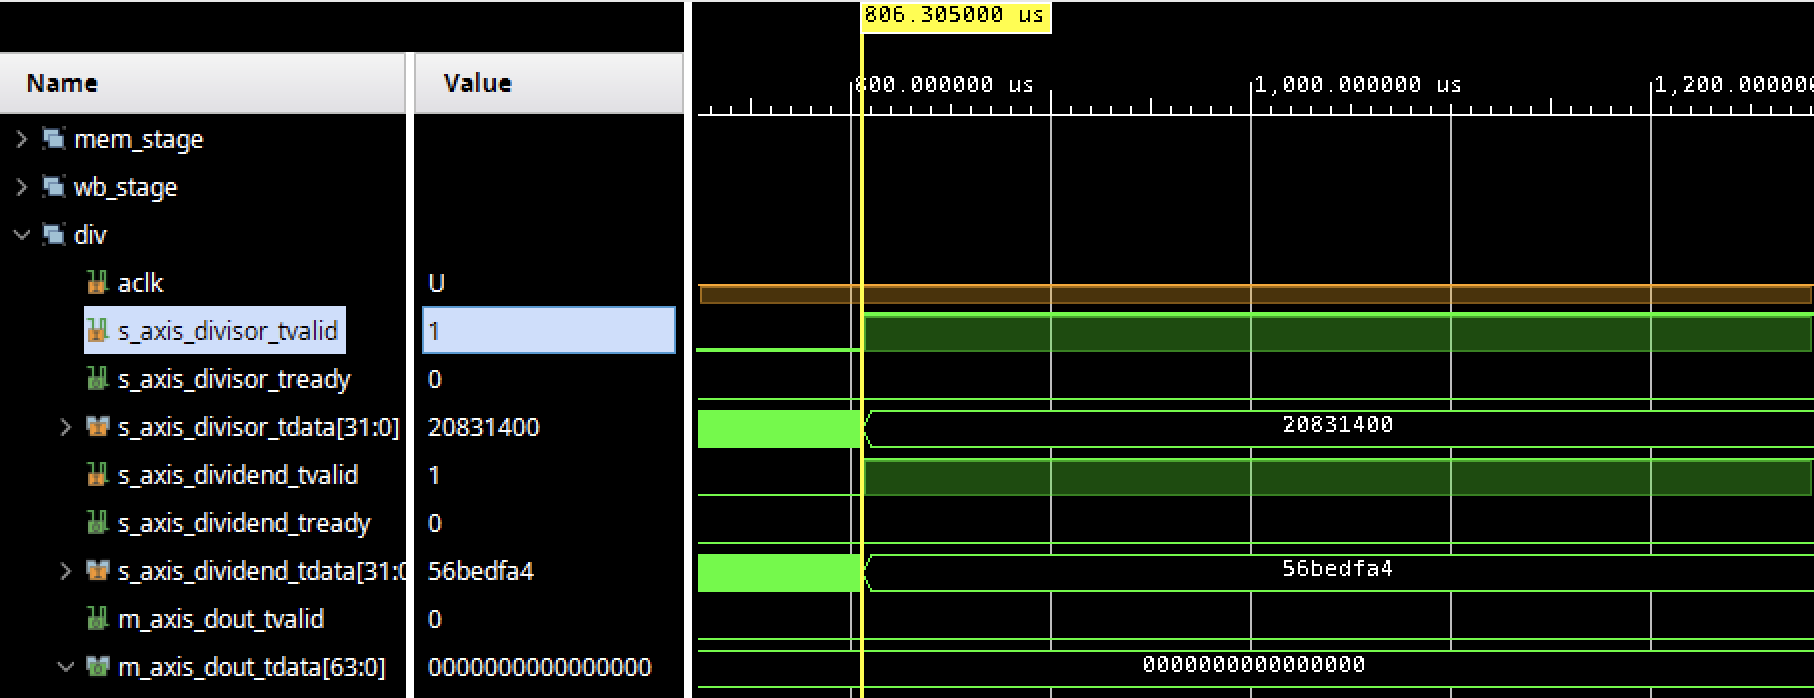
\includegraphics[width=0.85\linewidth]{no_aclk.png}
		\caption[no\_aclk]{除法器aclk信号悬空}
		\label{fig:noaclk}
	\end{figure}
	
	\subparagraph{分析定位过程 \& 错误原因}\hfill
	
	因为错误为除法指令,去查看div模块如何出错,发现一个未赋值信号
	
	\subparagraph{修正效果}\hfill
	
	只需要将div和divu模块接口全部定义就能避免这种问题
	
	\begin{lstlisting}[language=verilog]
	div_gen div(
		.aclk                   (clk),
		.s_axis_divisor_tdata   (alu_src2),
		.s_axis_dividend_tdata  (alu_src1),
		.s_axis_divisor_tready  (divisor_data_ready),
		.s_axis_dividend_tready (dividend_data_ready),
		.s_axis_divisor_tvalid  (div_data_valid),
		.s_axis_dividend_tvalid (div_data_valid),
		.m_axis_dout_tdata      (div_result),
		.m_axis_dout_tvalid     (div_res_valid)
	);
	\end{lstlisting}

	\subparagraph{总结归纳}\hfill
	
	今后在遇到新的模块进行例化时要将需要操作的接口看全、注意类型和位宽,恰当使用。
	
	\paragraph{错误\textbf{2.2:}除法器运算过程持续读取输入}\hfill
	
	\subparagraph{错误现象}\hfill
	
	在遇到一个除法指令后,Valid和Ready信号仍然同时拉高,读取除法器输入并进行运算,接连输出多个结果。后一条乘法指令的结果被覆盖导致错误。
	
	\begin{figure}[h]
		\centering
		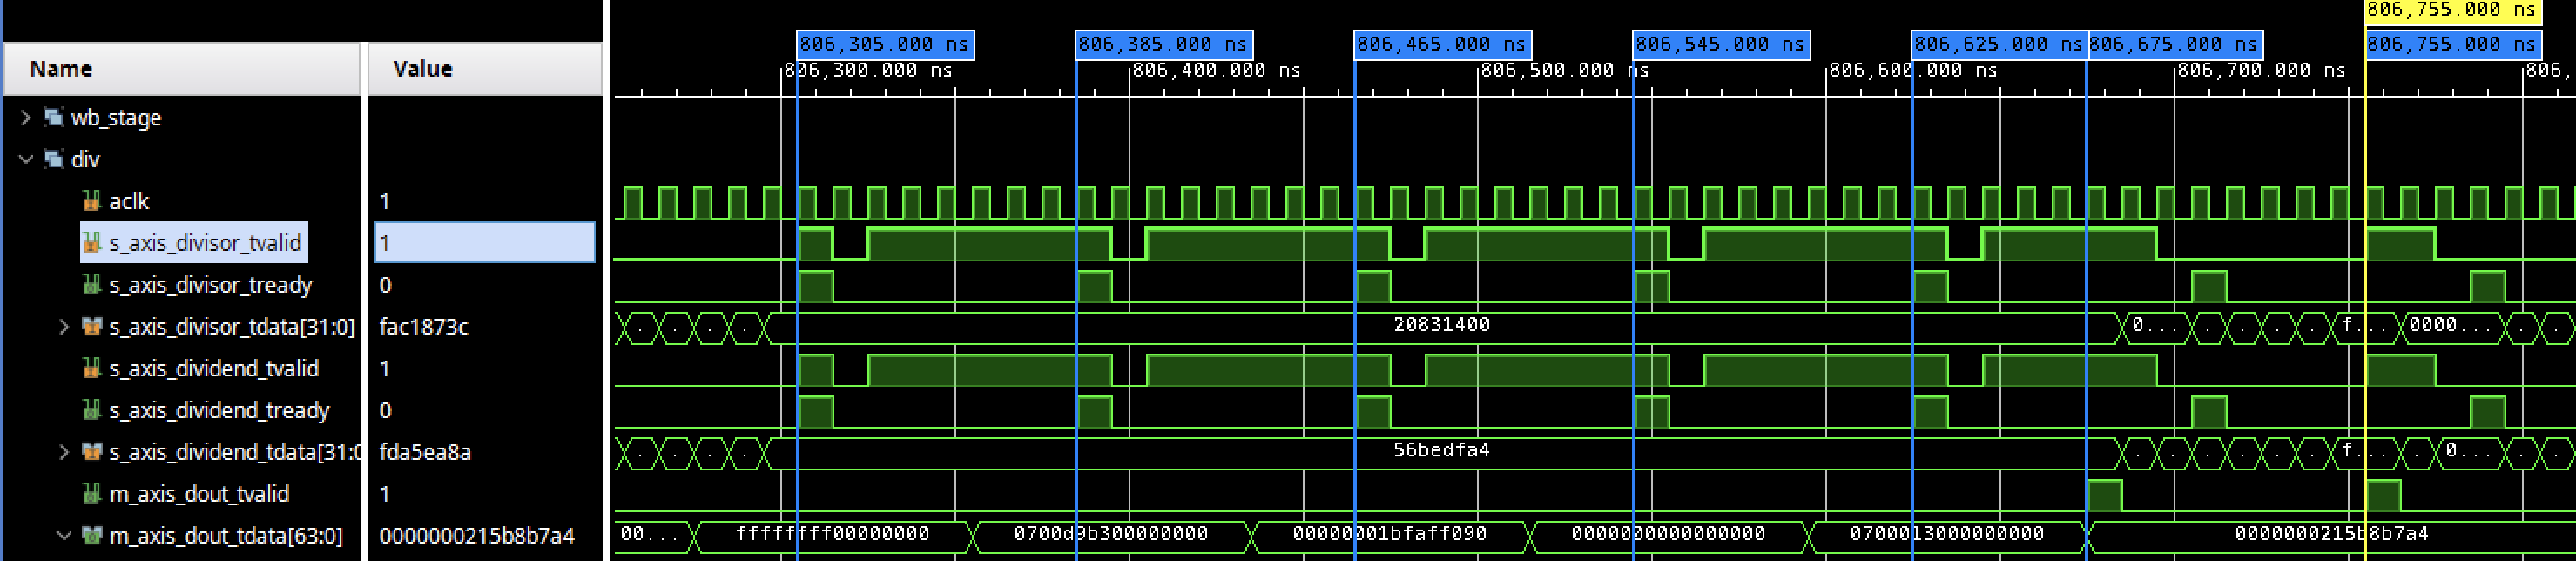
\includegraphics[width=1\linewidth]{valid_error.png}
		\caption[valid\_errpr]{除法器Valid信号设置错误}
		\label{fig:validerror}
	\end{figure}
	
	
	\subparagraph{分析定位过程}\hfill
	
	最初留意的现象是连续两次除法运算时,后一条指令Valid和Ready信号已经读取成功,但并不开始运算。与此同时,除法器结果和前一条除法指令相同,并且m\_axis\_dout\_tvalid信号为高电平。
	
	多次尝试分析后才理解讲义的意思,Valid信号并不是每遇到一次Ready就拉低,而是在一次除法过程中只能拉高一次,否则会持续读取输入进行运算。
	
	\subparagraph{错误原因}\hfill
	
	除法器Valid信号设置错误,在一次乘法指令中多次读取操作数输入进行运算,导致结果多次输出,可能会覆盖下一次乘法指令的结果。
	
	\begin{figure}[h]
		\centering
		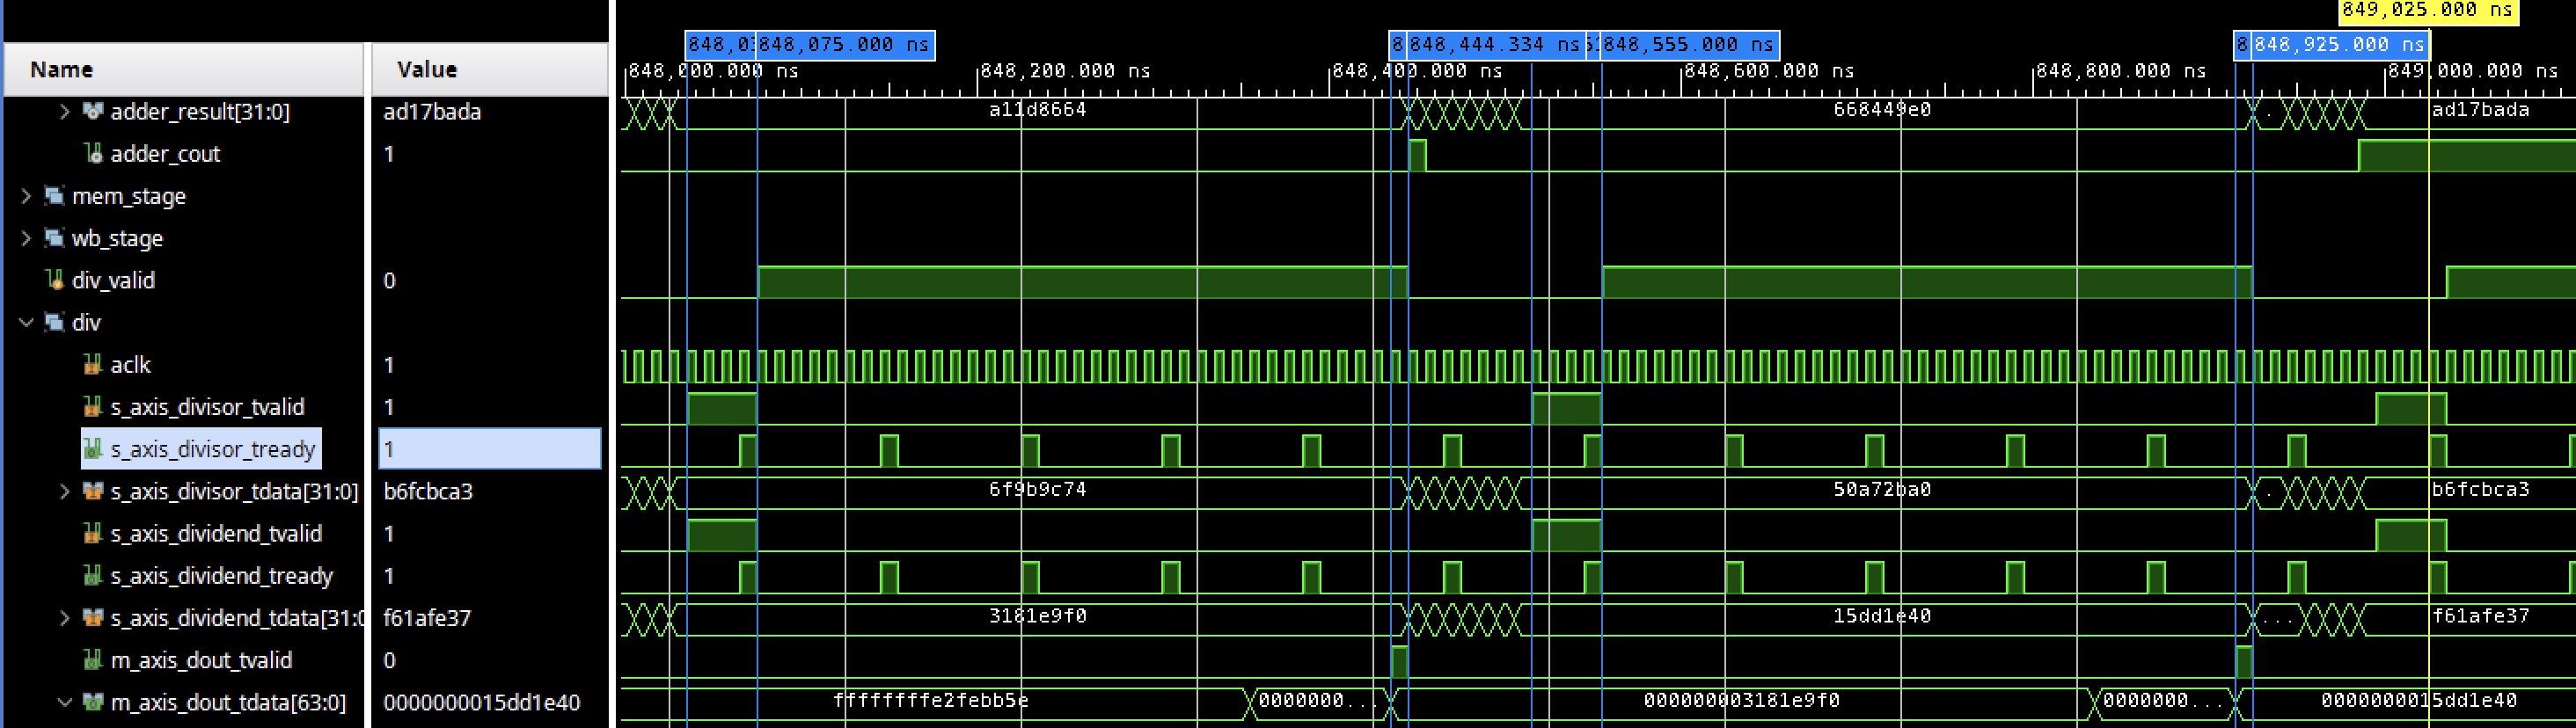
\includegraphics[width=1\linewidth]{valid_correct.png}
		\caption[Valid\_correct]{正确Valid输入信号效果}
		\label{fig:validcorrect}
	\end{figure}

	\subparagraph{修正效果}\hfill
	
	采用新的变量div\_valid来表示除法开始到结束的过程,在此过程中除法器Valid输入只能在最开始拉高,紧接着持续拉低,修正代码如\ref{Valid_input} 中代码所示。修正后效果如下页所示。
	
	\subparagraph{总结归纳}\hfill
	
	在遇到AXI总线多拍实现的部件时,需要对它输入输出接口的时序又深入了解,接合实现功能进行对接和赋值。
	
	\subsubsection{错误\textbf{3:}除法器设计实现错误}
	
	\paragraph{错误\textbf{3.1:}除法器中减法器清除窗口设置错误}
	
	\subparagraph{错误现象}\hfill
	
	第一个减法器即计算错误,上商为0按理不应该改变被除数,但是清除窗口将其改变为\texttt{64'h1}:
	
	\begin{figure}[h]
		\centering
		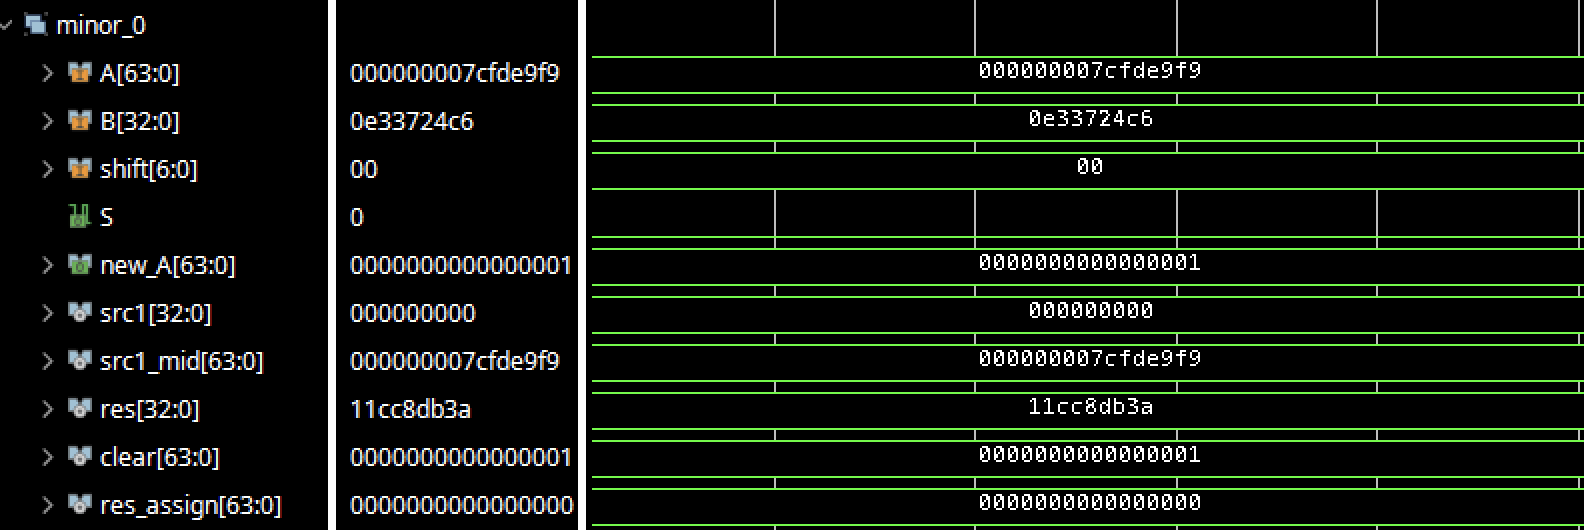
\includegraphics[width=0.85\linewidth]{figures/div_error_clear.png}
		\caption{清除窗口设置错误}
		\label{fig:diverrorclear}
	\end{figure}
	
	\subparagraph{分析定位过程}\hfill
	
	只需要仔细查看第一个减法器的信号即可发现主要错误是由\texttt{clear}清除信号引起,反查代码:
	
	\begin{lstlisting}[language=verilog]
		assign clear[63:0] = (S ? ((shift == 7'b0) ? {33'b0,31'h1} : {1'b1,33'b0,30'h1} >>> (shift-1)) : 64'h1);
	\end{lstlisting}

	发现明显错误,笔者本意是33个0和31个1拼起来,但实现起来却成了31位数1。
	
	\subparagraph{错误原因}\hfill
	
	减法器清除窗口设置错误,位拼接中位复制实现错误。
	
	\subparagraph{修正效果}\hfill
	
	正确实现目的即可,提供两种修改方案:
	
	\begin{lstlisting}[language=verilog]
		assign clear[63:0] = (S ? ((shift == 7'b0) ? {33'b0,{31{1'b1}}} : {1'b1,33'b0,{30{1'b1}}} >>> (shift-1)) : {64{1'b1}});
		
		assign clear[63:0] = (S ? ((shift == 7'b0) ? {33'b0,31'h7fffffff} : {1'b1,33'b0,30'h3fffffff} >>> (shift-1)) : 64'hffffffff);
		
		// both OK
	\end{lstlisting}
	
	\subparagraph{总结归纳}\hfill
	
	对于位复制和n位数的实现语法需要多记忆,属于低级错误。
	
	\paragraph{错误\textbf{3.2:}查找最高有效位算法实现错误}
	
	\subparagraph{错误现象}\hfill
	
	由于属于优化算法力度问题,在一些测试点并不会触发错误,但是某些测试点会出现结果错误,仔细反差,出错点及其之前的最高有效位计算结果错误。
	
	\begin{figure}[h]
		\centering
		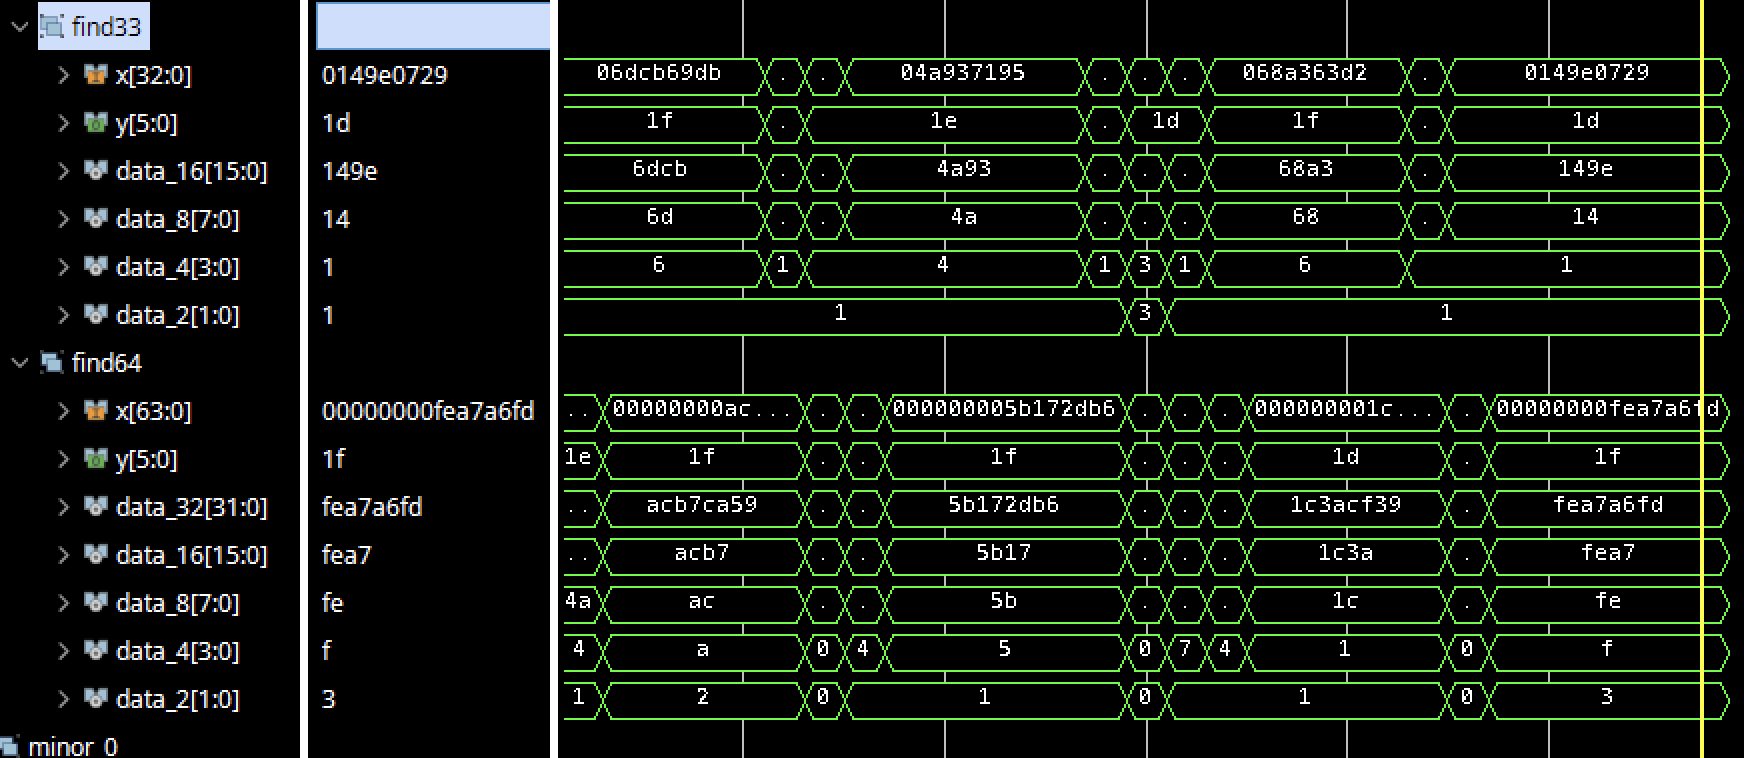
\includegraphics[width=0.85\linewidth]{figures/div_highest.png}
		\caption{查找最高有效位错误}
		\label{fig:divhighest}
	\end{figure}
	
	\subparagraph{分析定位过程}\hfill
	
	因为发现出错点加速初始化赋值过多,想到可能是最高有效位置差计算错误,查看最高有效位计算算法发现最后一位计算并不满足规律性特点,设计错误:
	
	\begin{lstlisting}[language=verilog]
		wire [31: 0]    data_32;
		wire [15: 0]    data_16;
		wire [ 7: 0]    data_8;
		wire [ 3: 0]    data_4;
		
		assign y[5] = |x[63:32];
		assign data_32 = y[5] ? x[63:32] : x[31:0];
		assign y[4] = |data_32[31:16];
		assign data_16 = y[4] ? data_32[31:16] : data_32[15:0];
		assign y[3] = |data_16[15:8];
		assign data_8  = y[3] ? data_16[15:8] : data_16[7:0];
		assign y[2] = |data_8[7:4];
		assign data_4  = y[2] ? data_8[7:4] : data_8[3:0];
		assign y[1] = |data_4[3:2];
		assign y[0] = |data_4[1:0];
	\end{lstlisting}
	
	仔细思考,\texttt{y[1],y[0]}的赋值并不满足算法。以为只要\texttt{y[1]}为1,则\texttt{data\_4}剩余位为0,\texttt{y[0]}不会取1。
	
	\subparagraph{错误原因}\hfill
	
	算法实现在末尾边界值错误,考虑轻率。
	
	\subparagraph{修正效果}\hfill
	
	根据算法及代码规律性,增加2位\texttt{data\_2}信号,重新计算末位:
	
	\begin{lstlisting}[language=verilog]
		wire [31: 0]    data_32;
		wire [15: 0]    data_16;
		wire [ 7: 0]    data_8;
		wire [ 3: 0]    data_4;
		wire [ 1: 0]    data_2;
		
		assign y[5] = |x[63:32];
		assign data_32 = y[5] ? x[63:32] : x[31:0];
		assign y[4] = |data_32[31:16];
		assign data_16 = y[4] ? data_32[31:16] : data_32[15:0];
		assign y[3] = |data_16[15:8];
		assign data_8  = y[3] ? data_16[15:8] : data_16[7:0];
		assign y[2] = |data_8[7:4];
		assign data_4  = y[2] ? data_8[7:4] : data_8[3:0];
		assign y[1] = |data_4[3:2];
		assign data_2  = y[1] ? data_4[3:2] : data_4[1:0];
		assign y[0] = data_2[1];
	\end{lstlisting}
	
	\subparagraph{总结归纳}\hfill
	
	对于设计算法的末尾边界计算情况不能想当然,需要考虑清晰。

	\subsubsection{错误\textbf{3:}访存操作存取半字控制信号错误}
	\paragraph{错误现象}\hfill
	
	%	四级节标题后面的\hfill与空行不可省略,不然节内容会跟着标题,目前我也只会这方法处理
	
	存访半字指令执行结果错误,标准结果为0x00004932:
	
	\begin{figure}[h]
		\centering
		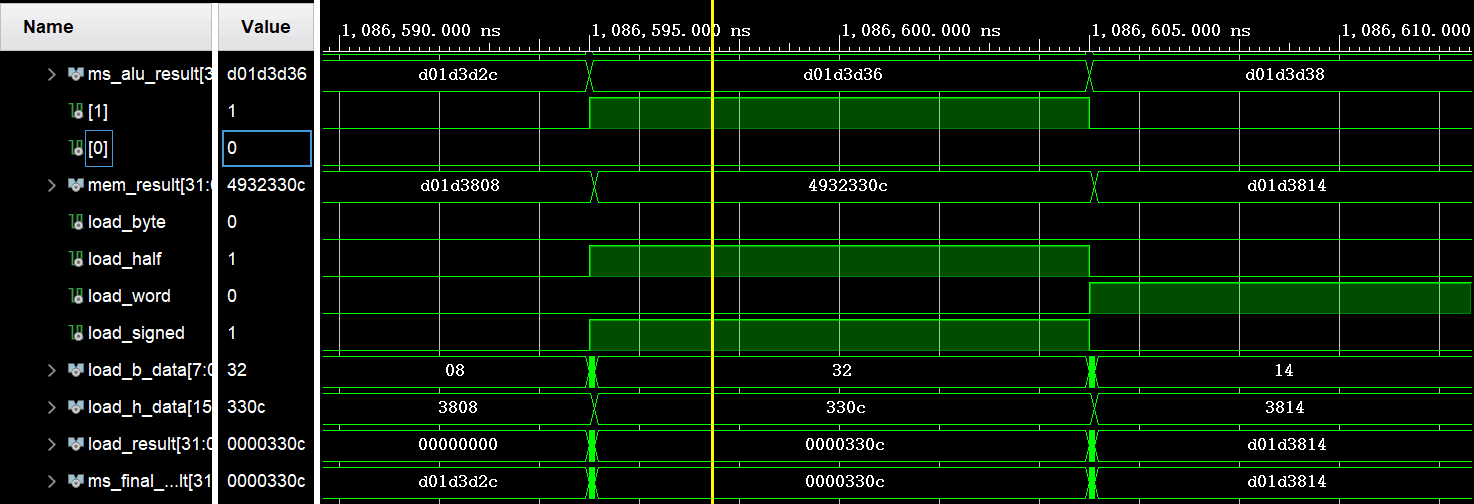
\includegraphics[width=0.85\linewidth]{figures/ldh_sth.png}
		\caption{存取半字控制信号错误}
		\label{fig:ldhsth}
	\end{figure}
	
	\paragraph{分析定位过程}\hfill
	
	咨询组员了解到存访半字使用的媒介控制信号为alu计算结果(访存地址的倒数第二位),而非最后一位。
	
	\paragraph{错误原因}\hfill
	
	存访半字控制信号使用错误,导致未能取到正确的半字。
	
	\begin{lstlisting}
		// store
		assign data_sram_wen   = 
				es_store_op[2] ? (4'h1 <<  es_alu_result[1:0])      : // b
				es_store_op[1] ? (4'h3 << es_alu_result[0]) : // h ERROR
				es_store_op[0] ? 4'hf : 4'h0;                          // w
		
		// load
		assign load_b_data = mem_result[{ms_alu_result[1:0], 3'b0}+:8];
		assign load_h_data = mem_result[ms_alu_result[0]+:16];	// h ERROR
		assign load_result = 
				{32{load_byte}} & {{24{load_b_data[ 7] & load_signed}}, load_b_data} |
				{32{load_half}} & {{16{load_h_data[15] & load_signed}}, load_h_data} |
				{32{load_word}} & mem_result;
	\end{lstlisting}
	
	\paragraph{修正效果}\hfill
	
	使用访存地址倒数第二位进行操作,\texttt{load, store}操作都需要改变:
	
	\begin{lstlisting}
		// store
		assign data_sram_wen 
			= es_store_op[2] ? (4'h1 <<  es_alu_result[1:0])      : // b
				es_store_op[1] ? (4'h3 << {es_alu_result[1], 1'b0}) : // h
				es_store_op[0] ? 4'hf : 4'h0;                          // w
												 
		// load
		assign load_b_data = mem_result[{ms_alu_result[1:0], 3'b0}+:8];
		assign load_h_data = mem_result[{ms_alu_result[1],   4'b0}+:16];
	\end{lstlisting}
	
	\paragraph{归纳总结}\hfill
	
	该问题由于设计经验和基础知识不足,讲义未明确说明存访半字使用的控制信息,今后会先查阅相关资料,了解设计原理和相关使用约定后进行设计实验。
	
	\section{实验总结}
	
	运算类指令的主要实现复用此前实现的数据通路,特别注意乘除法导致的时序问题即可,使用自行设计的乘除法器非常锻炼能力,并且当性能获得大幅度提升后成就感很高。转移、访存两类指令的大体实现思路同样基于已有的数据通路,具体实现细节上存在一定打磨钻研空间。
	
	时序满足上,(1)在除法器使用Xilinx IP时,乘法器使用Xilinx IP(即 * 号)时WNS为0.162\,ns,使用自行设计的单周期乘法器时WNS为0.073\,ns,将乘法器流水化后WNS(两拍完成乘法)为1.200\,ns;(2)在使用自行设计34拍除法器替换Xilinx IP,并在乘法器流水化条件下,WNS为0.008\,ns(3)当使用优化后的除法器,其余条件相同情况下,WNS为0.106\,ns。可见由于增加多个组合逻辑模块,且在硬件设计上未能充分优化,导致性能变差。
	
\end{document}